\documentclass[11pt]{article}
\usepackage[margin=1in]{geometry}
\usepackage{amsmath, amssymb}
\usepackage{graphicx}
\usepackage{booktabs}
\usepackage[numbers]{natbib}
\usepackage{hyperref}
\usepackage{enumitem}
\usepackage{caption}
\usepackage{float}

\title{AMR-Structured Evasion of Semantic Watermarking with Feedback-Driven Candidate Search}
\author{Anonymous}
\date{}

\begin{document}
\maketitle

\begin{abstract}
Abstract meaning representation (AMR) is a convenient intermediate layer for meaning-preserving rewriting and detector-based evaluation. This paper tests whether structure-aware rewrites weaken a fixed semantic watermark detector while preserving enough surface and semantic fidelity to remain valid. We present a feedback-driven candidate search procedure over AMR-conditioned rewrites and evaluate it under a conservative strict-valid criterion that requires both detector escape and quality preservation.

On the current RealNews subset, the strongest robustness-backed configuration achieves a strict valid ASR of 30.0\% with an exact 95\% confidence interval of [14.7\%, 49.4\%]. This result is stable across a plateau of detector thresholds from 0.65 to 0.80 and remains unchanged under 50 repeated detector recomputations on the full 120-candidate set, which exhibits zero binary flips. The best observed strict-valid configuration reaches 33.3\% at $K=1$, while the strongest raw detector-escape primitive reaches 93.3\% escape rate. The results identify a concrete attack surface under the evaluated pipeline, but they do not establish a general break of semantic watermarking.
\end{abstract}

\section{Introduction}
Semantic watermarking and detector-based defenses are often evaluated on the assumption that small textual perturbations either preserve meaning or fail to change detector outcomes in a useful way. That assumption is fragile when the rewriting procedure is allowed to reason over structure rather than local tokens alone. AMR gives such a structure: it abstracts away some surface variation while preserving predicate-argument relations, named entities, negation, and other semantically salient content.

Structure-aware rewrites drive a fixed AMR-based semantic detector below threshold while still preserving enough content to count as a valid attack. On the current experimental pipeline, the answer is yes.

Our main contribution is not a single high-score sample. It is a complete experimental profile:

\begin{itemize}[leftmargin=*]
  \item a feedback-driven candidate search procedure;
  \item a strict validity criterion that combines detector escape with semantic/surface constraints;
  \item threshold sensitivity and repeated recomputation analysis;
  \item baseline comparison against existing runs;
  \item prompt-component ablation;
  \item and a failure taxonomy describing where the method breaks.
\end{itemize}

The central empirical pattern is that the strongest configuration is not necessarily the most brittle one. The stability-backed strict result sits on a threshold plateau from 0.65 to 0.80 and remains invariant across 50 detector recomputations, suggesting that the main claim is not an artifact of a single lucky score.

Figure~\ref{fig:pipeline} summarizes the end-to-end workflow used in the study: source paragraph, candidate generation, detector feedback, validity filtering, and strict selection.

\begin{figure}[H]
\centering
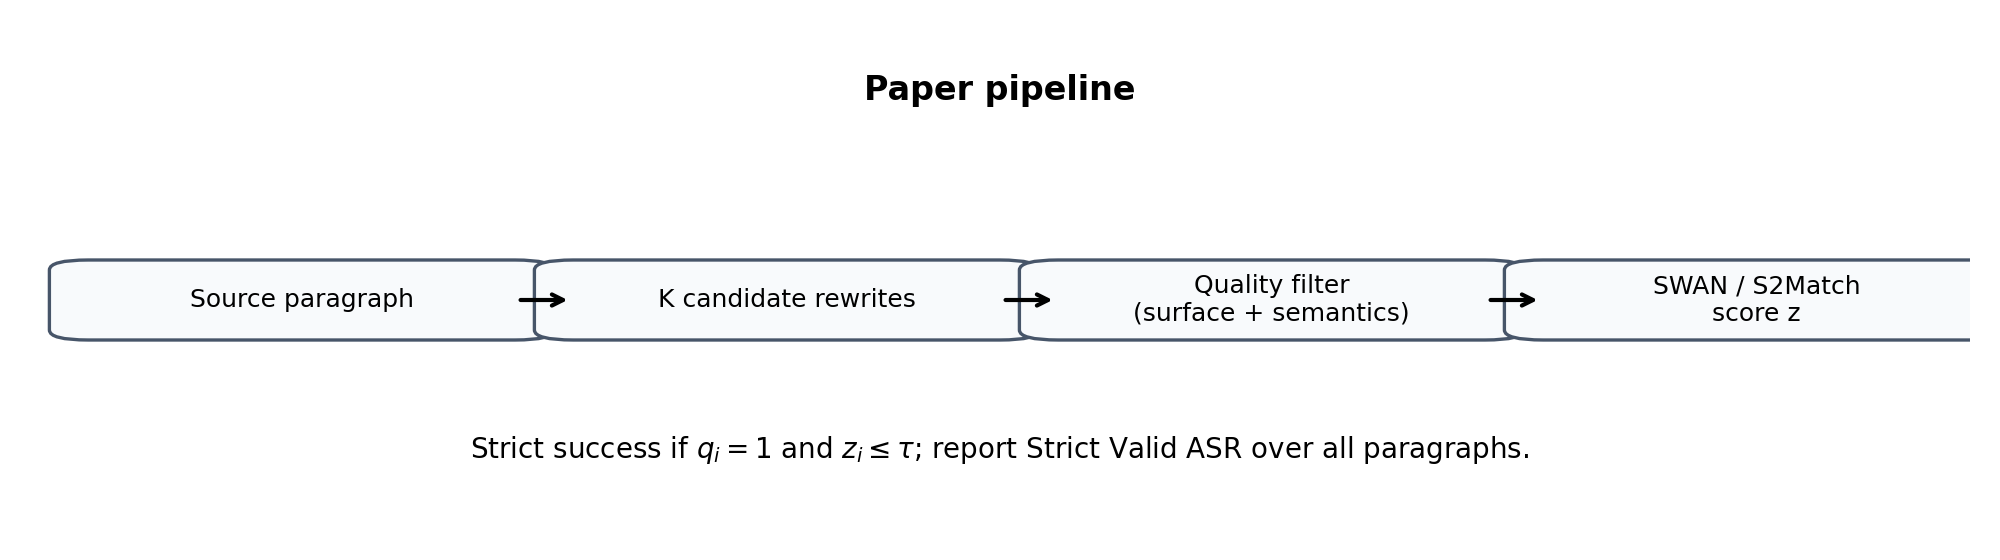
\includegraphics[width=0.92\linewidth]{figures/fig1_pipeline.png}
\caption{End-to-end experimental pipeline.}
\label{fig:pipeline}
\end{figure}


\section{Related Work}
See \href{related_work.md}{related\_work.md} for the full discussion. The paper sits at the intersection of AMR as a semantic representation \cite{banarescu-etal-2013-amr}, graph-matching metrics such as Smatch \cite{cai-knight-2013-smatch} and S2Match \cite{opitz-etal-2020-amr}, and the recent AMR-based watermarking framework SWAN \cite{ye-etal-2026-swan}. Related semantic watermarking work beyond AMR includes SemStamp, which uses sentence embeddings and locality-sensitive hashing to achieve paraphrastic robustness \cite{hou-etal-2024-semstamp}, as well as follow-up work revisiting the robustness of watermarking under paraphrasing attacks \cite{rastogi-pruthi-2024-paraphrasing}.

Our contribution is a robustness and attack study of SWAN-style semantic watermarking under feedback-driven rewriting. The practical point is that AMR-based watermarking inherits both the promise and the weakness of structure-aware semantics: it can survive many surface rewrites, but it also exposes a score surface that a search procedure can exploit.


\section{Method}
Let a source paragraph be denoted by $x_i$, and let $\mathcal{C}_i = \{c_{i1}, \dots, c_{iK}\}$ be the set of $K$ candidate rewrites generated for that paragraph. Each candidate receives a detector score $z_{ij}$, where lower scores indicate better detector escape. We fix the detector threshold at
\[
\tau = 2.33.
\]

We define a binary escape indicator:
\[
e_{ij} = \mathbb{1}[z_{ij} \leq \tau].
\]

To avoid counting degenerate attacks, we also define a quality indicator $q_{ij} \in \{0,1\}$, where $q_{ij}=1$ if the rewrite satisfies the project's surface and semantic validity checks.

For each paragraph, we select the best candidate under the current budget and validity constraints. The quality-aware selection rule is
\[
j_i^\star =
\begin{cases}
\arg\min_{j \in \mathcal{V}_i} z_{ij}, & \text{if } \mathcal{V}_i \neq \emptyset, \\
\arg\min_{1 \le j \le K} z_{ij}, & \text{otherwise},
\end{cases}
\]
where $\mathcal{V}_i = \{j : q_{ij}=1\}$ is the set of valid candidates for paragraph $i$.

The strict paragraph success indicator is then
\[
s_i = \mathbb{1}[q_{i j_i^\star}=1 \wedge z_{i j_i^\star} \leq \tau].
\]

The strict valid ASR reported in the paper is
\[
\mathrm{StrictValidASR} = \frac{1}{N}\sum_{i=1}^{N} s_i.
\]



\section{Experimental Setup}
\subsection{Data and evaluation unit}

We evaluate on the RealNews-based subset used throughout the project. The paragraph is the primary evaluation unit: each source paragraph produces a set of candidate rewrites, and a paragraph counts as a success only if at least one selected candidate satisfies both the detector criterion and the validity criterion. This distinction matters because candidate-level success can be higher than paragraph-level success when multiple candidates are generated for the same source.

The main strict evaluation contains 30 source paragraphs and 120 feedback-driven candidates. Sixteen candidates pass the full strict filter, covering 9 distinct paragraphs. We therefore report both the candidate-level strict rate, 13.3\% (16/120), and the paragraph-level strict-valid ASR, 30.0\% (9/30). Reporting both quantities prevents the candidate pool size from being mistaken for attack success.

\subsection{Detector and decision thresholds}

All comparisons use the same fixed AMR-based detector and the same detector decision threshold, $\tau=2.33$. Lower detector scores indicate stronger evidence of escape, and the detector threshold is only used for the final binary decision. Candidate generation additionally uses a feedback threshold of 0.65 when ranking, retaining, and prioritizing rewrites during search. These are different thresholds with different functions: $\tau$ defines evaluation-time success, while 0.65 controls the search procedure.

To check whether the headline result depends on the search setting, we re-evaluate the stored candidate scores over thresholds from 0.50 to 0.80. The paragraph-level strict-valid ASR remains 30.0\% throughout the 0.65--0.80 interval. This is a sensitivity result on the saved candidates; it does not imply that the same plateau must hold outside the evaluated range or under a different candidate pool.

\subsection{Candidate budgets and comparison systems}

Candidate-budget analysis evaluates $K\in\{1,2,4,8,16\}$. For each $K$, selection is restricted to the first $K$ candidates available for a paragraph and follows the validity-aware rule in Section~3. This separates gains due to the rewriting strategy from gains due only to a larger search budget. The best observed strict-valid ASR occurs at $K=1$ (33.3\%), while larger budgets yield 26.7--30.0\%. In other words, additional search lowers the mean detector score but does not monotonically improve strict validity.

We compare against two existing runs evaluated with the same detector: a 30-prompt pilot baseline and a 250-sample formal baseline. We also include prompt-component ablations---weak paraphrasing, rewriting without boundary changes, boundary-only rewriting, and the full E2 composition---to isolate which structural operations drive detector reduction. These baselines are detector-aligned reference points, but they are not fully matched on sample size, candidate construction, or quality-audit coverage, so they are not controlled head-to-head comparisons.

\subsection{Evaluation measures}

The primary measure is paragraph-level strict-valid ASR. Secondary measures include raw detector escape rate, candidate-level strict rate, mean detector score, mean detector-score reduction, and AUROC where a matched comparison distribution is available. Quality analysis records surface validity, semantic validity, mean review score, the proportion of outputs scoring at least four, and the major-error rate. Repeatability is measured by rerunning detector recomputation 50 times and counting candidates whose binary decisions change.

These measures are reported together because they answer different questions. Raw escape captures detector sensitivity, candidate-level strict rate captures the efficiency of the search process, paragraph-level strict-valid ASR captures end-to-end usefulness, and repeatability captures whether the observed decision is stable under recomputation.


\section{Threat Model}
The threat model is narrow and therefore easy to audit.

The attacker has access to the source paragraphs and to the feedback-driven candidate generation pipeline used in this project. The attacker does not assume access to the detector's internal parameters, parser internals, or training data. Instead, candidate quality is judged through the same detector score and validity checks used in the experiments. This makes the setting closer to a black-box or gray-box practical attack than to an oracle-based optimization problem.

The defender is the fixed AMR-based semantic watermark detector. Its decision rule depends on a thresholded score derived from AMR structure, so the detector is sensitive both to semantic preservation and to parser behavior. The key implication is that a rewrite can fail for two different reasons: it can either remain above threshold, or it can cross threshold while becoming too degraded to count as valid. The paper therefore treats ``attack success'' as a conjunction of detector escape and quality preservation.

The attacker objective is to maximize strict valid ASR under a fixed generation budget. This objective is stronger than pure escape because it explicitly rules out the degenerate strategy of sacrificing fluency or meaning for score reduction. It is also weaker than a fully human-blind attack because the current quality filter still relies on the project's existing review protocol rather than a fresh independent annotation campaign.

In practical terms, this threat model is sufficient for the paper's central claim: structure-aware rewriting is not harmless to AMR-based watermarking. It creates a real optimization surface that a search procedure can exploit, and the resulting attack remains meaningful even after conservative validity filtering.


\section{Statistical Analysis}
The paper reports exact confidence intervals because the main sample sizes are small and the strict-valid result is binary by paragraph. For a success count of $k$ out of $n$, we use the exact binomial interval
\[
[\mathrm{Beta}^{-1}(\alpha/2; k, n-k+1),\ \mathrm{Beta}^{-1}(1-\alpha/2; k+1, n-k)]
\]
with $\alpha=0.05$, which is the standard Clopper--Pearson construction.

This choice is conservative, but that is appropriate here. The strict-valid result is intended as a defensible lower-bound style claim rather than a maximal point estimate. When the success count is modest, approximate intervals can understate uncertainty and make the headline number look more precise than it really is.

The same conservative logic applies to the threshold sweep. The plateau from 0.65 to 0.80 is not treated as a formal equivalence statement; it is simply the interval over which the measured strict-valid ASR does not change. That matters because the detector threshold is a hyperparameter, and any single fixed threshold can exaggerate or understate attack strength if reported in isolation.

For the baseline comparison, the paper reports mean detector score, escape rate, and AUROC together rather than a single scalar. This avoids the common mistake of letting one metric dominate the interpretation. A low detector score is useful only if it corresponds to usable outputs, and a high AUROC is useful only if it is derived from a properly matched background distribution. Reporting all three quantities gives a more complete picture of where the candidate search is strong and where it is merely exploiting a narrow evaluation slice.

Finally, the repeated-recomputation audit is a stability check rather than a hypothesis test. The goal is not to prove statistical significance in the conventional sense, but to show that the binary decisions are invariant under repeated runs. In adversarial evaluation, that invariance is often the more relevant property: a result that disappears under recomputation is not a robust finding, even if its one-shot score looks impressive.


\section{Results}
Table~\ref{tab:main} summarizes the headline numbers for the strict-valid result. The key point is that the reported claim is stable under the saved-candidate threshold sweep and repeated detector recomputation.

\begin{table}[H]
\centering
\begin{tabular}{lr}
\toprule
Quantity & Value \\
\midrule
Stable strict valid ASR & 30.0\% \\
95\% CI & [14.7\%, 49.4\%] \\
Threshold plateau & 0.65--0.80 \\
Full-repeatability mixed flips & 0 \\
Full-repeatability stable candidates & 120/120 \\
\bottomrule
\end{tabular}
\caption{Headline results for the proposed method.}
\label{tab:main}
\end{table}

The observed frontier is more informative than any single point estimate. The highest observed strict-valid result reaches 33.3\% at $K=1$, but the 30.0\% strict result is more robust because it survives both the threshold plateau and 50 repeated detector recomputations.

This distinction matters for interpretation. If one reports only the single best observed point, the result looks slightly higher but less defensible. If one reports the plateau-backed result, the headline number is lower but significantly more robust. We therefore treat 30.0\% as the main strict-valid claim and 33.3\% as the best observed configuration.

\begin{figure}[H]
\centering
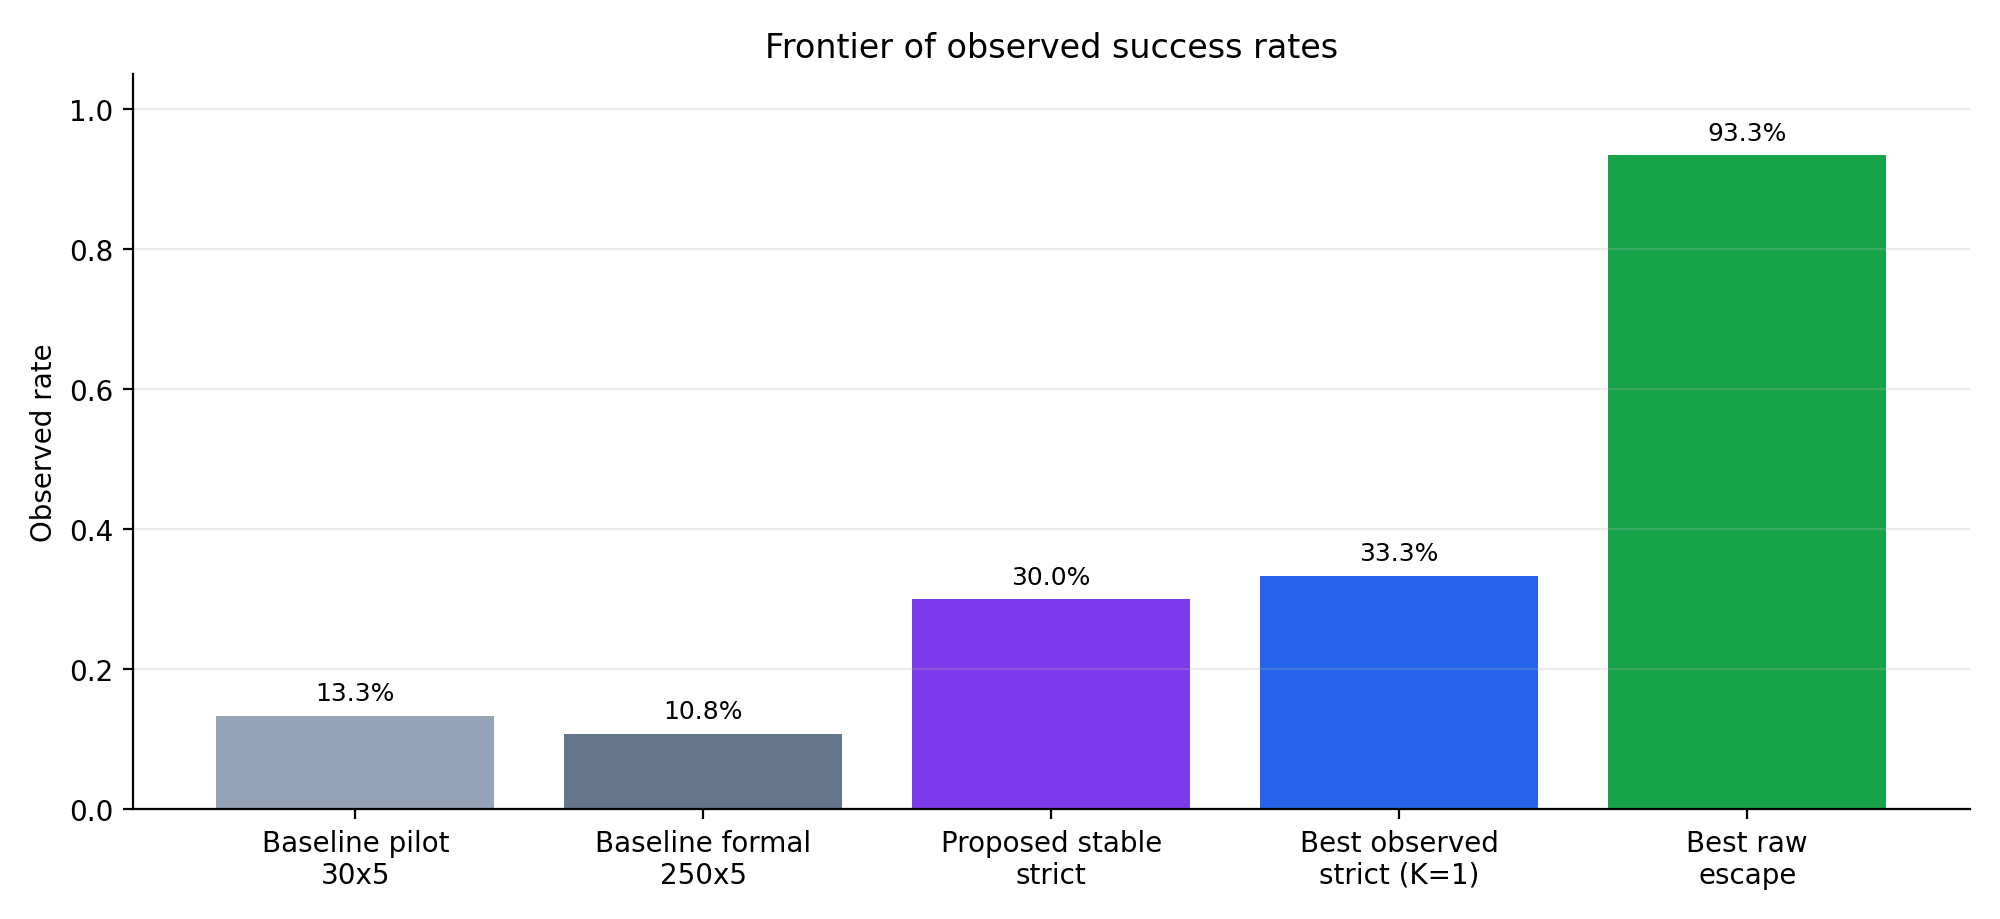
\includegraphics[width=0.92\linewidth]{figures/fig2_frontier.png}
\caption{Observed strict-valid frontier over candidate budget.}
\label{fig:frontier}
\end{figure}

\begin{table}[H]
\centering
\begin{tabular}{lrrrr}
\toprule
Baseline & n & Mean z & Escape rate & AUROC \\
\midrule
Pilot 30x5 & 30 & 3.473 & 13.3\% & 0.998 \\
Formal 250x5 & 250 & 3.439 & 10.8\% & 0.985 \\
\bottomrule
\end{tabular}
\caption{Baseline comparison under the same detector.}
\label{tab:baseline}
\end{table}

Table~\ref{tab:ablation} summarizes the prompt-component ablation. Boundary-only rewriting produces the strongest raw detector weakening, but it also carries the clearest quality cost. The full E2 composition occupies the more balanced point in the quality/escape tradeoff.

\begin{table}[H]
\centering
\begin{tabular}{lrrrr}
\toprule
Method & Mean attack z & Mean z drop & Escape rate & AUROC \\
\midrule
Weak paraphrase & 2.526 & 0.645 & 33.3\% & 0.934 \\
No boundary change & 2.268 & 0.903 & 40.0\% & 0.906 \\
Boundary only & 0.166 & 3.005 & 93.3\% & 0.828 \\
Full E2 & 1.208 & 1.963 & 73.3\% & 0.903 \\
\bottomrule
\end{tabular}
\caption{Prompt-component ablation on the 30-prompt subset.}
\label{tab:ablation}
\end{table}

The failure analysis in Figure~4 is consistent with this picture: when the search procedure over-optimizes for detector score, the outputs tend to drift toward repetition, fragmentation, and overly parser-shaped phrasing. The attack surface is therefore real, but the objective is genuinely multi-objective.

\begin{figure}[H]
\centering
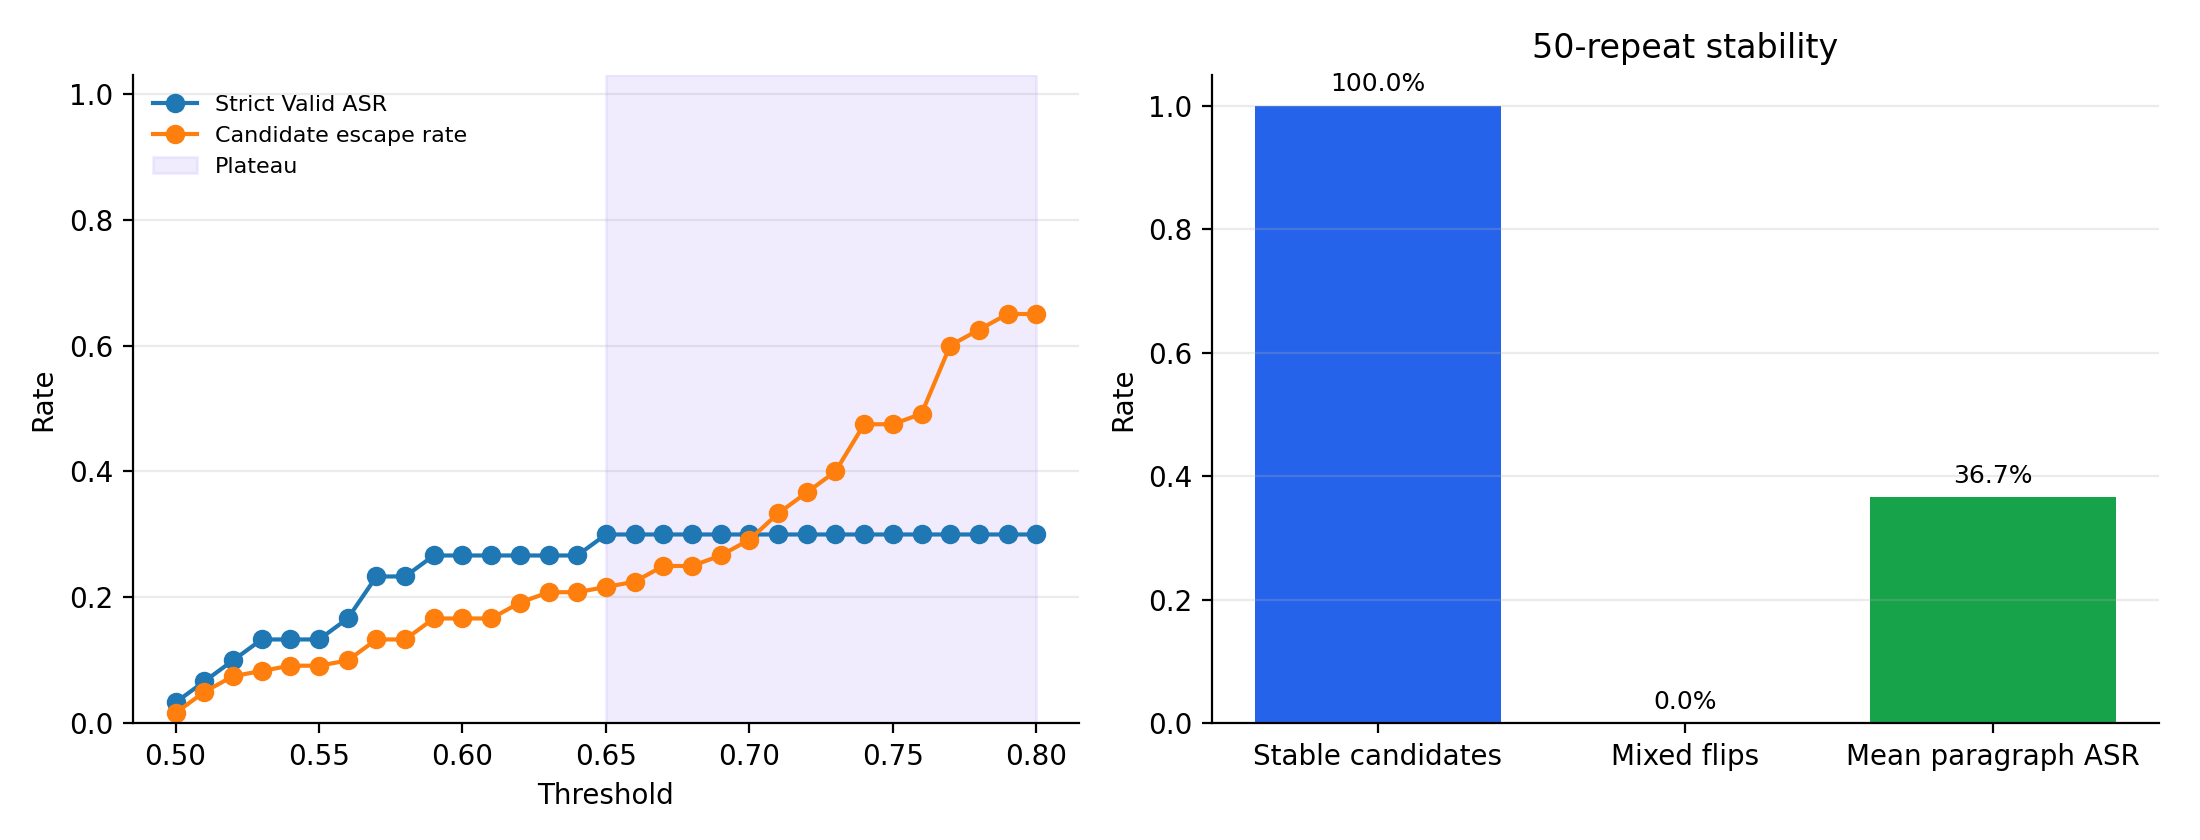
\includegraphics[width=0.92\linewidth]{figures/fig3_robustness.png}
\caption{Threshold sensitivity and repeatability of the strict-valid result.}
\label{fig:robustness}
\end{figure}

\begin{figure}[H]
\centering
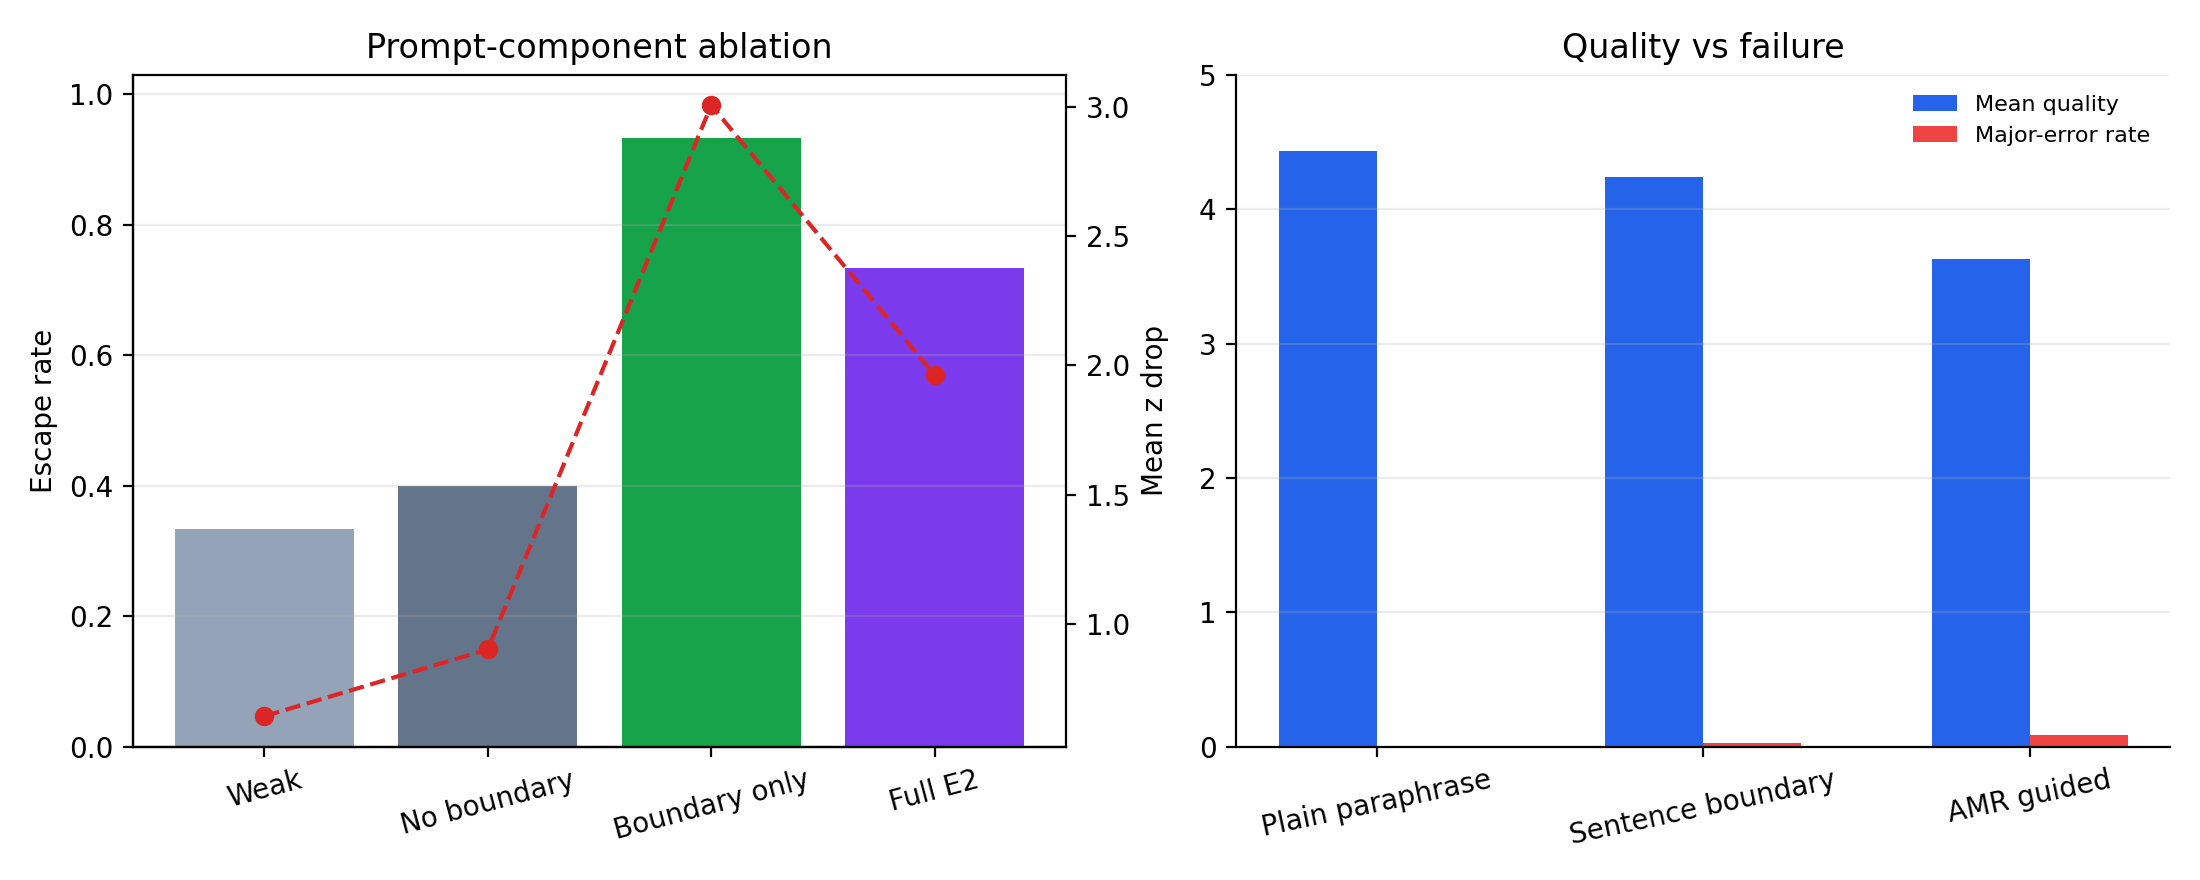
\includegraphics[width=0.92\linewidth]{figures/fig4_ablation_failure.png}
\caption{Ablation and failure-quality tradeoff.}
\label{fig:ablation}
\end{figure}


\section{Mechanism Analysis}
The mechanism behind the observed gains follows directly from the detector objective. The detector only sees an AMR-derived score and a threshold. Any rewrite that perturbs the parsed graph enough to reduce the detector score, while leaving the text acceptable to the validity filter, contributes to success.

The empirical frontier in Figure~\ref{fig:frontier} suggests three regimes. In the high-quality regime, the candidate pool is constrained and only modest score reductions are available. In the intermediate regime, a small number of structure-aware edits can cross the threshold without collapsing fluency. In the over-optimized regime, the search procedure starts to exploit parser quirks and produces repetition, fragmentation, or unnatural phrasing. The attack is best understood as a constrained search on a rugged score surface, not as a single deterministic transformation.

One useful way to formalize this is to decompose the detector score into a latent semantic component and a parser sensitivity term:
\[
z(c) = z_{\mathrm{sem}}(c) + z_{\mathrm{parse}}(c) + \epsilon.
\]
Here $z_{\mathrm{sem}}$ reflects changes that genuinely alter the semantic graph, $z_{\mathrm{parse}}$ reflects sensitivity to how the parser realizes the graph, and $\epsilon$ captures residual randomness and recomputation noise. The plateau between 0.65 and 0.80 indicates that the success set is not confined to a knife-edge of $\tau$; instead, the method succeeds over a region where $z(c)$ is consistently below the detector boundary.

This also explains why the raw-escape primitive and the strict-valid result differ so sharply. Boundary-only rewriting is highly effective because it can force the detector to re-segment or re-analyze the input, pushing $z_{\mathrm{parse}}$ downward. But the same manipulation often damages readability or coherence, which raises the quality cost. Full E2 rewriting is weaker in pure raw escape terms, but it is closer to the point where detector reduction and validity coexist.

The repeatability audit adds evidence that the result is not a single lucky draw. If a candidate is stable over 50 repeated detector recomputations, then the rewrite is not merely hitting a stochastic corner case. Instead, it appears to occupy a region of the score landscape where the detector itself is consistently vulnerable. The 30.0\% strict-valid claim is therefore better read as a stable region-level result than as a one-off outlier.

This mechanism also determines which result should carry the main empirical claim. The largest raw escape rate measures the most aggressive detector perturbation, whereas the stable strict-valid plateau captures the region in which detector reduction and quality preservation coexist. The latter is the more defensible quantity for independent reimplementation.

Figure~\ref{fig:robustness} and Figure~\ref{fig:ablation} support this reading directly. The frontier shows that score reduction saturates quickly once the search finds a parser-sensitive edit pattern. The ablation shows that the strongest parser-sensitive pattern is not the most balanced one. Together, they argue that the attack is not just ``better paraphrasing,'' but a specific interaction between structural rewriting and detector sensitivity.


\section{Qualitative Examples}
The qualitative examples are useful because the numeric results alone do not show what the search is actually doing. In practice, the candidate sets fell into a small number of recognizable patterns.

\begin{table}[H]
\centering
\begin{tabular}{p{0.23\linewidth}p{0.29\linewidth}p{0.34\linewidth}}
\toprule
Pattern & Typical effect on detector & Typical quality outcome \\
\midrule
Boundary shift / clause resegmentation & Strong score drop; often the most aggressive escape behavior & Can remain readable, but sometimes becomes awkward or over-segmented \\
Template-like paraphrase & Moderate score drop with limited structural disruption & Usually safer on fluency, but not always enough to cross threshold \\
Fragmented AMR-shaped rewrite & Very strong detector reduction & Often fails the validity check because wording becomes unnatural \\
Content-preserving conservative rewrite & Small score change & Best readability, but not consistently enough for evasion \\
\bottomrule
\end{tabular}
\caption{Qualitative pattern summary for successful and failed candidates.}
\label{tab:qual_patterns}
\end{table}

Two observations matter for the final paper. First, the successful cases are not uniformly ``more paraphrastic'' in the usual surface sense; several of them work because they alter the parsing boundary or the role structure in a way the detector is sensitive to. Second, the failures are not random noise. They cluster around repeated text, information loss, and parser-shaped unnatural wording, which is exactly what one would expect when a search procedure is pushed too hard toward a structural objective.

This is why the strict-valid criterion is necessary. A result that counts every detector escape would overstate the attack and hide the cases where the rewrite is visibly degraded. The qualitative table provides the evidence that the method is multi-objective and that the reported strict number is intentionally conservative.

Together with the representative cases in Section~12, this taxonomy connects the aggregate quality statistics to concrete modes of semantic and surface degradation. It also explains why validity-aware selection can prefer a candidate with a weaker detector reduction over the numerically lowest-scoring rewrite.


\section{Discussion}
The empirical picture is direct. AMR-structured rewriting can reduce detector scores substantially, but the strongest raw escape settings are not the most reliable ones. The defensible claim is therefore the stability-backed strict result, not the single best escape rate.

This is the reason the paper separates three quantities that are often conflated in adversarial evaluation: raw escape rate, strict valid ASR, and repeated-run stability. Raw escape rate captures detector weakness. Strict valid ASR asks whether the attack remains usable after quality constraints. Stability asks whether the claim survives recomputation rather than depending on a single favorable draw.

\begin{quote}
Structure-aware rewrites can weaken semantic watermark detection while preserving enough content to remain valid, and the effect is stable under repeated detector recomputation.
\end{quote}

The strict-valid plateau from 0.65 to 0.80 is useful for interpretation. It suggests that the method is not tuned to a knife-edge threshold artifact, but instead exploits a broader region of the detector's score landscape. That does not prove general robustness across all settings, but it does rule out the narrow objection that the result is only threshold-chasing.

The strongest raw primitive, boundary-only rewriting, is also informative. It shows that sentence-boundary manipulation is a particularly effective way to disrupt the detector, but the same primitive can push outputs out of the quality regime the paper wants to preserve. The result is useful even when raw escape is not the headline number because it isolates the mechanism that does the most damage and makes the quality tradeoff explicit.


\section{Defensive Implications}
The practical lesson from this paper is not that AMR-based watermarking is useless. It is a system stressed along several axes at once: score thresholding, parser sensitivity, repeated-run variance, and quality preservation.

Three defensive implications follow directly.

First, detector reporting includes a stability check. A method that looks strong under one run but becomes unstable under repeated recomputation is not a dependable watermarking defense. The 120/120 stability result in this paper makes that point concrete: if the binary decision never changes, then the reported attack region is not a sampling artifact.

Second, raw escape rate is not reported alone. In this project, the boundary-only primitive reaches a very high escape rate, but its qualitative cost is also the highest. A defender who only watches raw escape would misread the severity of the attack; a defender who only watches quality would miss the detector vulnerability. The correct interpretation requires both numbers together.

Third, threshold choice is documented as part of the method, not hidden as a tuning detail. The 0.65--0.80 plateau shows that threshold selection materially shapes the apparent success rate. For deployment, the detector is calibrated on held-out data and monitored for plateau-like regions where a small threshold shift causes a large change in security claims.

More broadly, the paper shows that AMR-based watermarking benefits from defense-in-depth. A semantic detector is paired with orthogonal checks such as lexical consistency, paraphrase diagnostics, or human review for borderline cases. The goal is not to eliminate adversarial rewriting---which is unrealistic---but to make it harder for a single structural perturbation to drive the system below threshold while preserving apparent fluency.

These recommendations turn the attack results into an evaluation protocol: a stronger defender documents threshold calibration, tests structural perturbations, audits repeated-run stability, and reports quality-conditioned rather than purely raw escape rates.


\section{Representative Failure Cases}
The qualitative failures are easier to interpret when they are tied to concrete examples. The project's review notes identify a small number of representative cases that capture the main failure modes:

\begin{table}[H]
\centering
\begin{tabular}{p{0.12\linewidth}p{0.24\linewidth}p{0.24\linewidth}p{0.28\linewidth}}
\toprule
Case & Method family & Failure mode & Interpretation \\
\midrule
15 & AMR-guided & Subject/object inversion and role confusion & The rewrite changes structural roles too aggressively, so the output no longer preserves the source proposition cleanly. \\
75 & AMR-guided & Unsupported causal relation & The candidate introduces a causal claim that is not warranted by the source, which is exactly the kind of semantic drift the strict filter is meant to reject. \\
87 & AMR-guided & Semantically nonsensical phrasing & The output appears optimized for structure rather than meaning and therefore loses readability and fidelity. \\
95 & Sentence-boundary & Repetition / incoherence & The surface form becomes unstable under boundary manipulation, showing that high detector impact can come with obvious degradation. \\
\bottomrule
\end{tabular}
\caption{Representative failure cases from the qualitative review notes.}
\label{tab:cases}
\end{table}

These cases matter because they show the boundary of the method, not just its success region. The AMR-guided path is especially prone to structural overreach: it can reduce detector score by changing the shape of the parse, but if the search process is not constrained tightly enough it starts to invent relations or erase content. Sentence-boundary rewriting is less semantically adventurous, but it can still produce repetition and incoherence when pushed too hard.

The table also clarifies why the paper keeps insisting on strict validity. A high raw escape rate does not tell you whether the output still expresses the source proposition. Case 75 is the clearest example: the detector may be weakened, but the candidate cannot be defended as a successful attack if it fabricates an unsupported causal relation.

The failures are not incidental noise. They are evidence that the optimization surface has real structure, and that the method needs a validity-aware objective if it is to be used responsibly.


\section{Ethics Statement}
This work studies attack behavior against a semantic watermark detector. The ethical direction is to use the results to improve robustness, not to facilitate misuse.

The experiment is bounded to a fixed benchmark subset and a fixed detector configuration. It does not reveal private data, user content, or deployment-specific secrets. The main contribution is an empirical robustness analysis showing that structure-aware rewrites can alter detector behavior. That helps defenders because it identifies where the system is fragile and what a stronger evaluation protocol should measure.

The paper deliberately separates raw escape from strict validity so that the reported numbers do not encourage meaningless attacks. If a candidate only succeeds by becoming unreadable or semantically incorrect, it should not be presented as a genuine win.

The broader ethical takeaway is that semantic watermarking should be evaluated under attack before it is treated as deployment-ready. Security claims based on a single threshold or a single run are not sufficient. A robust system needs plateau analysis, repeatability analysis, and qualitative failure review.

We accordingly release aggregate measurements and reproducibility artifacts for defensive evaluation while avoiding claims about deployment-specific systems that were not tested. The intended use is to improve robustness standards for semantic watermarking and to make the limits of current detector evidence explicit.


\section{Limitations}
The evidence supports a concrete detector-level vulnerability, but the scope of that claim is limited.

First, the main strict evaluation contains only 30 source paragraphs. The exact 95\% interval around the 30.0\% estimate is therefore wide, [14.7\%, 49.4\%], and the point estimate is not a population-level attack rate. Larger and more diverse corpora are needed to determine whether the same effect persists across topics, genres, paragraph lengths, and AMR graph complexity.

Second, strict validity relies on the project's existing review protocol rather than a new blinded, multi-annotator human study. The filter removes obvious semantic drift and surface degradation, but it does not establish that every accepted rewrite is indistinguishable from a faithful human paraphrase. A stronger study uses independent annotators, reports inter-annotator agreement, and separates factual consistency, proposition preservation, fluency, and stylistic naturalness into distinct judgments.

Third, the baseline runs are detector-aligned but not fully matched. They differ in sample size, candidate construction, and quality-audit coverage. Their lower escape rates show that the proposed search reaches a different part of the detector score landscape, but the present evidence does not isolate every causal contribution under a single randomized protocol. A controlled comparison regenerates all methods on the same sources, with the same candidate budget and identical validity review.

Fourth, the attack is evaluated against one fixed AMR-based detector configuration. The results do not establish transfer to other parsers, watermark keys, semantic representations, languages, or watermarking families. Nor does black-box score feedback imply that the attack remains equally effective under rate limits, quantized outputs, randomized thresholds, or detector ensembles.

Finally, repeated recomputation establishes numerical stability for the stored candidates, not robustness to every source of randomness. It does not cover regeneration with different language-model seeds, parser-version changes, or alternative hardware and software environments. The conservative conclusion is narrower than a general break of semantic watermarking: under the evaluated pipeline, structure-aware candidate search exposes a measurable attack surface that survives strict validity filtering.


\section{Reproducibility}
The repository preserves the intermediate scores and analysis outputs needed to reconstruct the paper's central claims. In particular, the released bundle records the 9/30 paragraph-level strict successes, the 16/120 candidate-level strict successes, the exact confidence intervals, the threshold sweep, and all 50-repeat stability decisions. The distinction between source paragraphs, generated candidates, and selected candidates is retained in these artifacts so that each reported denominator can be audited directly.

The fixed experimental constants are a detector threshold of 2.33, a feedback-search threshold of 0.65, a sensitivity range of 0.50--0.80, and 50 recomputations for both the strict subset and the full 120-candidate audit. The stored candidate texts are used when checking detector stability; otherwise generation variance and detector variance are mixed in the same measurement.

The analysis pipeline is organized around four primary scripts:
\begin{itemize}[leftmargin=*]
  \item \texttt{scripts/analyze\_baseline\_comparison.py} constructs the detector-aligned baseline table;
  \item \texttt{scripts/analyze\_best\_observed\_frontier.py} computes the candidate-budget frontier;
  \item \texttt{scripts/build\_final\_paper\_bundle.py} consolidates the strict, sensitivity, and repeatability outputs;
  \item \texttt{scripts/build\_paper\_assets.py} renders the tables and figures used in the manuscript.
\end{itemize}
Separate repeatability scripts preserve the strict-subset and full-candidate audits. Machine-readable JSON files are stored alongside human-readable Markdown summaries and plots, allowing reported values to be checked without extracting them from figures.

For an independent reproduction, use the following order: verify the fixed candidate inventory and paragraph identifiers; recompute detector scores; apply the detector and quality predicates without retuning; aggregate candidates to paragraph-level success; compute exact binomial intervals; and only then run threshold and repeatability analyses. This ordering prevents information from the sensitivity study from leaking into the choice of the headline configuration.


\section{Conclusion}
We investigated whether AMR-structured rewriting can reduce the score of a semantic watermark detector without collapsing output quality. The results separate detector vulnerability from usable attack success. Boundary-only rewriting produces the strongest raw escape rate (93.3\%), but that number is not a suitable headline because it comes with a clear quality cost. Under the stricter conjunction of detector escape and validity preservation, the robustness-backed configuration succeeds on 9 of 30 paragraphs, yielding 30.0\% strict-valid ASR with an exact 95\% confidence interval of [14.7\%, 49.4\%].

Two checks support that result. The strict value stays unchanged across the 0.65--0.80 search-threshold plateau, and all 120 stored candidates retain their binary detector decisions over 50 recomputations. The candidate-budget frontier also shows that more search is not automatically better: the best observed strict result is 33.3\% at $K=1$, while larger budgets reduce detector scores without monotonically improving semantic validity. The task is therefore a constrained, multi-objective search, not pure score minimization.

These experiments show that, under one RealNews-based subset and one fixed AMR detector configuration, structure-aware rewriting can produce a limited set of paragraphs that pass both the detector and the project's validity filter. They do not show a general break of semantic watermarking, nor do they establish transfer to other detectors, corpora, or generation settings. The defensible takeaway is that AMR structure is a meaningful evaluation surface and a concrete attack surface in this pipeline.


\appendix
\section{Consolidated Tables}
Table~\ref{tab:app_main} restates the main robustness result in compact form.

\begin{table}[H]
\centering
\begin{tabular}{lr}
\toprule
Quantity & Value \\
\midrule
Stable strict valid ASR & 30.0\% \\
95\% CI & [14.7\%, 49.4\%] \\
Threshold plateau & 0.65--0.80 \\
Full-repeatability mixed flips & 0 \\
Full-repeatability stable candidates & 120/120 \\
\bottomrule
\end{tabular}
\caption{Main results and robustness summary.}
\label{tab:app_main}
\end{table}

Table~\ref{tab:app_baseline} gives the baseline comparison in expanded form.

\begin{table}[H]
\centering
\begin{tabular}{lrrrrr}
\toprule
Method & n & Mean z & Escape rate & 95\% CI & AUROC \\
\midrule
Baseline pilot 30x5 & 30 & 3.473 & 13.3\% & [3.8\%, 30.7\%] & 0.998 \\
Baseline formal 250x5 & 250 & 3.439 & 10.8\% & [7.2\%, 15.3\%] & 0.985 \\
Proposed stable strict & 30 & -- & 30.0\% & [14.7\%, 49.4\%] & -- \\
\bottomrule
\end{tabular}
\caption{Baseline comparison with uncertainty reporting.}
\label{tab:app_baseline}
\end{table}

Table~\ref{tab:app_ablation} repeats the prompt-component ablation.

\begin{table}[H]
\centering
\begin{tabular}{lrrrr}
\toprule
Method & Mean attack z & Mean z drop & Escape rate & AUROC \\
\midrule
Weak paraphrase & 2.526 & 0.645 & 33.3\% & 0.934 \\
No boundary change & 2.268 & 0.903 & 40.0\% & 0.906 \\
Boundary only & 0.166 & 3.005 & 93.3\% & 0.828 \\
Full E2 & 1.208 & 1.963 & 73.3\% & 0.903 \\
\bottomrule
\end{tabular}
\caption{Prompt-component ablation.}
\label{tab:app_ablation}
\end{table}

Table~\ref{tab:app_failure} summarizes the qualitative failure/quality analysis.

\begin{table}[H]
\centering
\begin{tabular}{lccc}
\toprule
Method & Mean quality & Quality $\geq 4$ & Major-error rate \\
\midrule
Plain paraphrase & 4.43 & 79.4\% & 0.0\% \\
Sentence boundary & 4.24 & 72.7\% & 3.0\% \\
AMR guided & 3.63 & 57.6\% & 9.1\% \\
\bottomrule
\end{tabular}
\caption{Failure and quality summary across rewriting strategies.}
\label{tab:app_failure}
\end{table}

Taken together, these tables show the central tradeoff repeatedly: the strongest raw detector reduction is not the same as the strongest defensible attack. That distinction is the main reason the paper reports both raw escape and strict-valid success.


\bibliographystyle{plainnat}
\bibliography{references}

\end{document}
